\clearpage
\fancyhead[R]{\small\color{muted}Vulkan · Sun Temple}
\section{神庙长廊}
入口两旁的雕像背对廊灯，翅膀边缘比身体亮。沿地面的红色镶边向里看，石柱从偏暖的浅灰逐渐过渡到冷灰。这里保留了 Epic Games 随模型提供的入口机位，布光则在 Redflag 中重新安排。前厅和长廊各有自己的点光源，调整其中一盏，就能在这条连续的地面上看到影响范围。

\begin{figure}[H]\centering
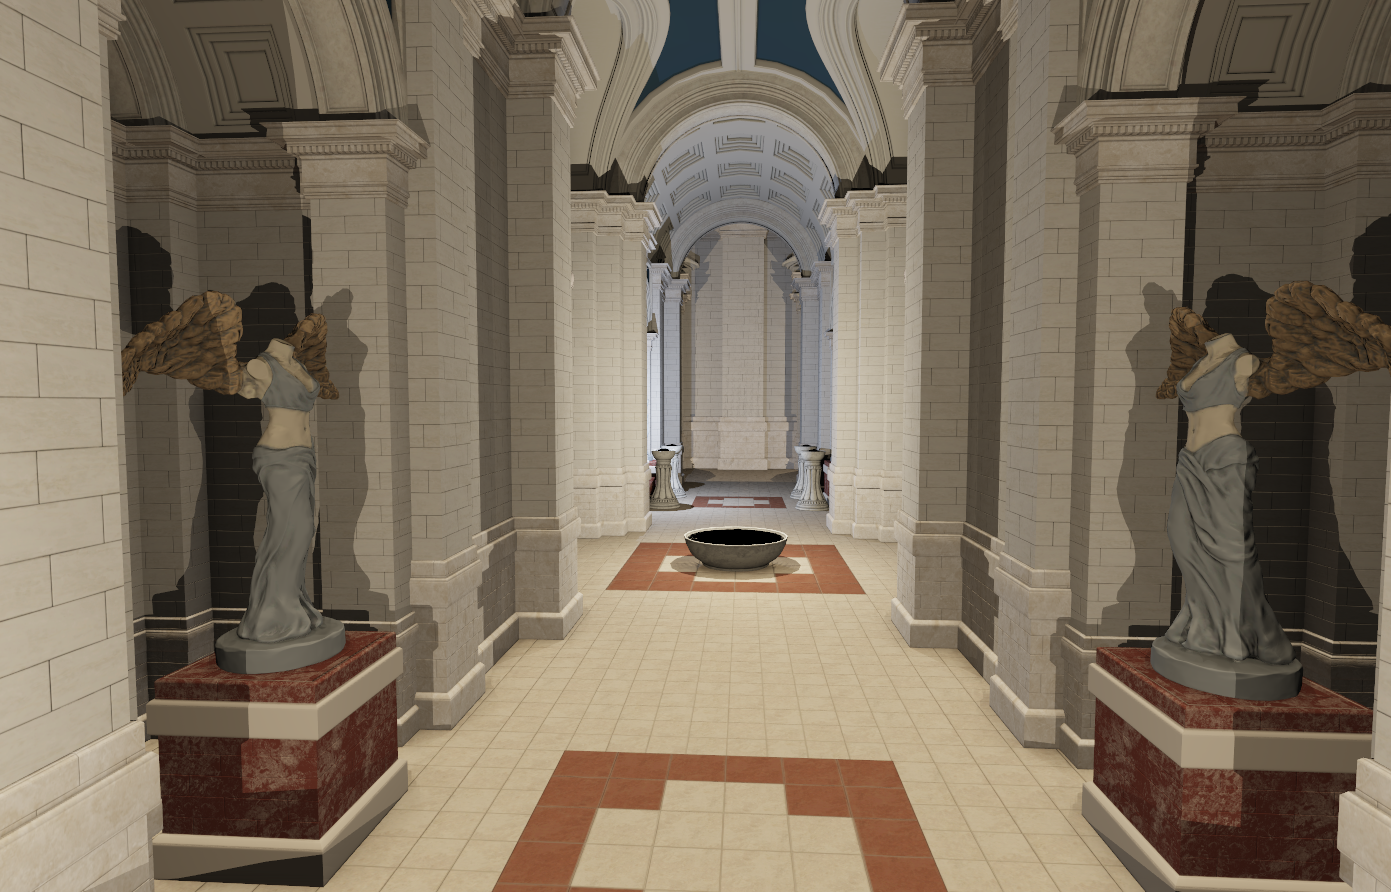
\includegraphics[width=.96\linewidth]{sun-temple/SunTemple.png}
\caption{Redflag 的 Vulkan 视口，第 12 帧。图中使用全部八盏点光源，以及 DDGI、GTAO 和 TAA。场景原图为 $1391\times892$ 像素，从编辑器实际提交给 ImGui 的图像导出。}
\end{figure}

第一次打开前，在仓库根目录运行 \path{python tests/fetch_sun_temple.py}。脚本需要 Blender 5、Pillow 和 NumPy。它检查原始压缩包，把静态建筑变成编辑器能加载的 glTF，再把 DDS 贴图转换为 PNG。回到编辑器，在项目面板双击 \path{Sun-Temple.redflag}。选中「前厅灯」调低强度，雕像旁的地砖会先暗下去，长廊后半段仍受另外几盏灯照亮。想保留这个改动，保存场景即可。

原始模型包含 517 件静态物体。它们仍保持各自的位置；为了减少重复加载相同材质，准备脚本按材质将几何合为 48 组，共 606,376 个三角形。这批模型和图像来自 Epic Games，由 Kai-Hwa Yao 与 Nicholas Hull 从 Unreal Engine 导出并发布在 NVIDIA ORCA，许可为 CC BY-NC-SA 4.0。

\par\noindent\source{https://developer.nvidia.com/ue4-sun-temple}{NVIDIA ORCA · Sun Temple}
\quad\source{https://creativecommons.org/licenses/by-nc-sa/4.0/}{模型与配图许可}
\quad\href{run:../scenes/sun-temple/README.md}{导入方法与截帧记录}

\clearpage
\section{火盆上的余烬}
走近神庙墙角的火盆，盆沿和石柱都受房间里的灯照亮。盆里的炭也有自己的颜色。模型给它附了一张自发光贴图，只有细小的炭纹发红。旧版导入了火盆，却漏读了这张图，所以房间的灯再亮，盆中也少了这层红色。

\begin{figure}[H]\centering
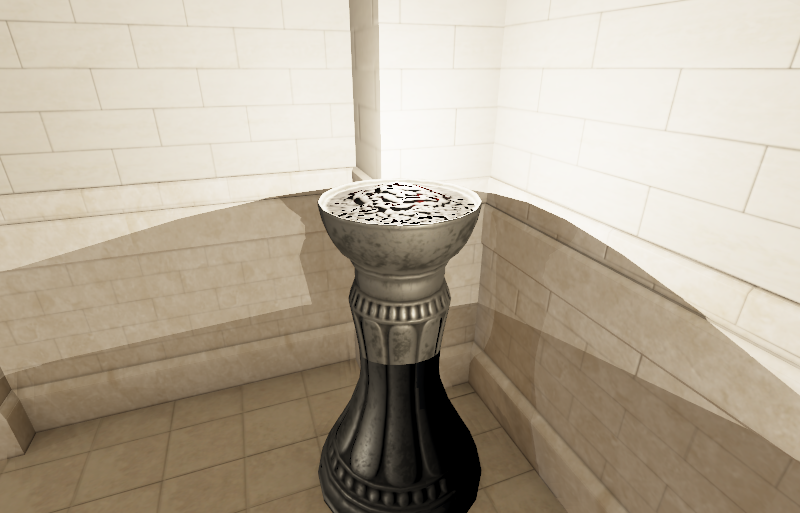
\includegraphics[width=.75\linewidth]{../../../output/profiling/emissive-studio/temple.png}\\[5pt]
\begin{minipage}{.47\linewidth}\centering
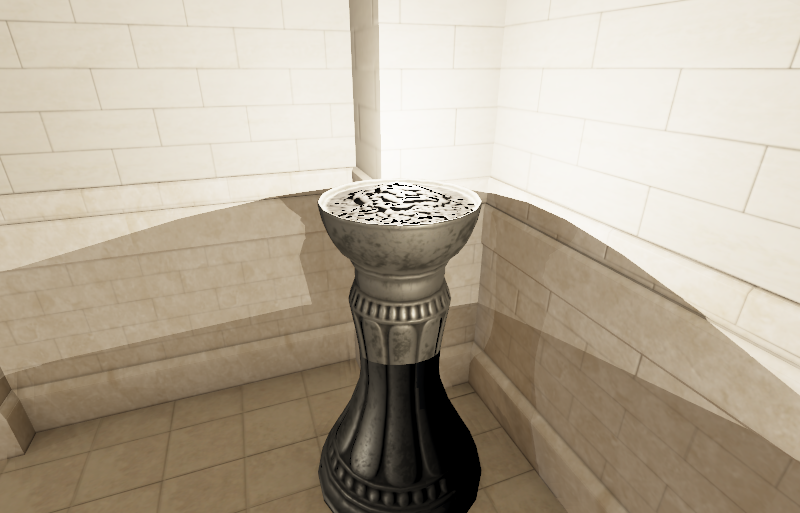
\includegraphics[width=\linewidth,trim=310bp 278bp 310bp 172bp,clip]{../../../output/profiling/emissive-studio/temple-before.png}\\旧版\end{minipage}\hfill
\begin{minipage}{.47\linewidth}\centering
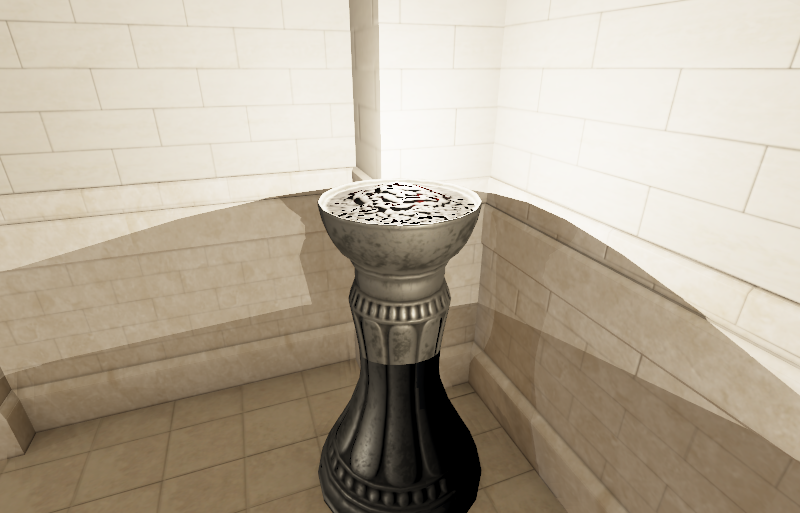
\includegraphics[width=\linewidth,trim=310bp 278bp 310bp 172bp,clip]{../../../output/profiling/emissive-studio/temple.png}\\读入自发光以后\end{minipage}
\caption{上图是 Redflag Vulkan 编辑器中的火盆。下排放大同一块盆面，保留编辑器原来的颜色。两次截帧使用同一机位、同一组灯和相同的曝光。}
\end{figure}

最明显的一处在原图坐标 $(419,202)$，从左上角开始计数。显示器还没有调整亮度时，这里的红色从 0.274 增至 0.878，绿色只从 0.214 变为 0.216。整张图中，红色增量超过 0.1 的只有 104 个像素。因此比较这种细小材质时，要把盆面放大，并读回原来的颜色。整幅画面的平均亮度很难告诉我们炭纹有没有画出来。

\source{https://developer.nvidia.com/ue4-sun-temple}{模型与贴图：Epic Games / NVIDIA ORCA}
\quad\href{run:../profiling/emissive-studio/README.md}{相机、截帧与测量方法}
